% !TeX spellcheck = de_CH
\documentclass[a4paper]{scrartcl}

\usepackage[T1]{fontenc}
\usepackage[utf8]{inputenc}
\usepackage[english, ngerman]{babel} 
\usepackage{tabu}
\tabulinesep=1.2mm

% Mathematik
\usepackage{amsmath}
\usepackage{amssymb}
\usepackage{amsfonts}
\usepackage{enumitem}

% Images
\usepackage{graphicx}
\graphicspath{{img/}} % default paths
 
% Shortcuts
\newcommand{\abl}[2]{\frac{\text{d}}{\text{d}#2}\text{ } #1 \text{ }\mathrm{d}t}
 
%opening
\title{PhAI Cheatsheet Draft}
\author{Fabian Hauser}

\begin{document}

\maketitle

\begin{abstract}
	Dieses Dokument gibt einen Überblick über die PhAI-Vorlesung FS2017
\end{abstract}

%TODO: Ableitungsregeln, Cos/Sin etc.

\section{Kinematik}
	\begin{tabu} {l X}
		\hline
		Gleichförmige Bewegung
		&	$s(t) = v \cdot t + s_0$ 
		\\
		&	$\vec{v}$ (Konstant)
		\\ \hline
		Gleichmässig beschleunigte
		&	$s(t) = \frac{1}{2} a \cdot t^2 + v_0 \cdot t + s_0$
		\\
		Bewegung
		&	$\vec{v}(t) = \vec{a} \cdot t + \vec{v}_0$
		\\
		&	$\vec{a}$ (Konstant)
		\\ \hline
		Mittlere Geschwindigkeit
		&	$\bar{v} = \frac{\Delta s}{\Delta t} = \frac{s_2 - s_1}{t_2 - t_1}$
		\\ \hline
		Mittlere Beschleunigung
		&	$\bar{a} = \frac{\Delta v}{\Delta t}$ 
		\\ \hline
	\end{tabu}

\section{Kinetik}
	\begin{tabu} {l X l}
		\hline
		Impuls
		&	$\vec{p} = \left[ Ns \right] = \left[ \frac{kg \cdot m}{s} \right]$	%TODO: Impuls m \cdot v?
		& 
		\\ \hline
		Kraft
		&	$\vec{F}=m\vec{a} = \left[ N \right] = \left[ \frac{kg \cdot m}{s^2} \right] = \abl{\vec{p}}{t}$ (Newtonscher Impulssatz) %TODO: RLY?
		&	Newton
		\\ \hline
		Energie
		&	$W = \left[ J \right] = \left[ N m \right] = \left[ Ws \right] = \left[ \frac{kg \cdot m^2}{s^2} \right]$
		&	Joule
		\\
		&	$1 \left[kWh\right] = 3.6 \cdot 10^6 \left[ J \right]$
		&
		\\ \hline
		Leistung
		&	$P = \left[ W \right] = \left[ \frac{J}{s} \right] = \left[ \frac{kg \cdot m^2}{s^3} \right]$
		&	Watt
		\\ \hline
	\end{tabu}
	
\subsubsection{Kinetische Energie}
	\begin{tabu} {l X}
		Kraft & $F = ma = \frac{p}{t}$ \\
		Strecke & $s = \frac{1}{2} a t^2$ \\
		Geschwindigkeit & $v = at$ \\
		Beschleunigung & $a$\\
		Impuls & $p = mv$ \\
		Energie & $W = Fs = \frac{1}{2} mv^2$
	\end{tabu}
			
	\begin{figure}[h]
		\centering
		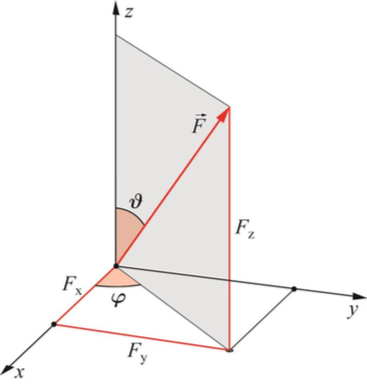
\includegraphics[width=0.3\linewidth]{img/darstellungKraefte.png}
		\caption{Darstellung von Kräften}
		\label{fig:darstellungkraefte}
	\end{figure}
		\begin{tabu} {l X}
			\multicolumn{2}{l}{2 Dimensional} \\
			$F_x = $ & $Fcos(\alpha)$ \\
			$F_y = $ & $Fsin(\alpha)$ \\
			\multicolumn{2}{l}{3 Dimensional} \\
			$F_x = $ & $Fcos(\varphi)sin(\vartheta)$ \\
			$F_y = $ & $Fsin(\varphi)sin(\vartheta)$ \\
			$F_z = $ & $Fcos(\vartheta)$
		\end{tabu}
			\begin{tabu} {l X}
				\multicolumn{2}{l}{Berechnung trigonometrische Funktionen} \\
				$sin(\alpha) = $ & $\frac{Gegenkathete}{Hypotenuse}$ \\
				$cos(\alpha) = $ & $\frac{Ankathete}{Hypotenuse}$ \\
				$tan(\alpha) = $ & $\frac{Gegenkathete}{Ankathete}$ = $\frac{sin(\alpha)}{cos(\alpha)}$
			\end{tabu}

\subsubsection{Potentielle Energie}

\begin{tabu} {l X}
	Kraft & $F = mg = \frac{p}{t}$ \\
	Höhe & $h = \left[ m \right]$ \\
	Geschwindigkeit & $v = gt$ \\
	Beschleunigung & $g \approx 9.81 \frac{m}{s^2}$ \\
	Impuls & $p = mv$ \\
	Energie & $W = Fh = mgh$
\end{tabu}

\subsubsection{Federkraft}

	
	\begin{tabu} {l X}
		Federkonstante & $k = \left[ \frac{N}{m} \right] = \left[ \frac{kg}{s^2} \right]$ \\
		Kraft & $F = kx$ \\ %TODO: Was ist $x$?
		Energie & $	W = \frac{1}{2} k x^2$
	\end{tabu}
	

\subsection{Schiefer Wurf}
	%TODO: Schiefer Wurf
	%SW02 Slide 34

\subsection{Haft- und Gleitreibung}
	Ist unabhängig von der Fläche.
	
	%TODO: Schiefe Ebene
	
	
	\paragraph{Gleichgewicht eines starren Körpers an der Ebene}
	$F_{tot} = \sum{F_i} = 0$
	%TODO: Slide 26 Vorlesung


\subsection{Drehmoment}
	Drehmoment wird in $t^{-1}$, meist $\text{s}^{-1}$ oder $\text{min}^{-1}$ angegeben.
	
	Die Hebelkraft funktioniert dank dem Drehmoment.

\subsection{Winkelgeschwindigkeit und Radialbeschleunigung}
	Die Winkelgeschwindigkeit wird in $\omega = \frac{v}{r}\left[ \frac{rad}{s} \right]$ angegeben
	
	Winkelbeschleunigung wird mit mit $\alpha$ angegeben.
	
	Die Radialbeschleunigung zeigt nach innen zum Kreismittelpunkt
	
	Berechnung: $a_r = \omega^2 r = \frac{v^2}{r} = \left[ \frac{rad}{s^2} \right]$

\subsubsection{Rotationsenergie}

	Rotationsenergie: $W = E_{rot} = \frac{1}{2} J \omega^2$
	%TODO: Slide 3, Freitag 21.04.
	
\subsubsection{Impuls}

Impulserhaltung: In einem geschlossenen System ohne externe einflüsse ist der Impuls 0. 
	
\subsubsection{Drehimpuls} %TODO: Übersichtlicher in Tabelle?
	Der Drehimpuls $L$ ist parallel zur Drehachse. Um diesen zu ändern, braucht es einen Drehmoment.

	$L = \sum_i{r_i \times p_i} = \sum_i{r_i \times mv_i}$
	$\left[ L \right] = kg m^2 s^{-2}$
	
	$\frac{dL}{dt} = M \Rightarrow \frac{d\overline{p}}{dt} = \overline{F}$
	
	%TODO: Screenshot Slide 8


	\paragraph{Drehimpulserhaltung}
	
	Die Energie aus einem Drehimpuls muss erhalten bleiben.
	
	
	\paragraph{Drehimpuls auf der schiefen Ebene} \hfill \\
	
	Runde Zylinder, welche eine schiefe Ebene hinunterrollen: $mgh = E_{kin} + E_{rot} =\frac{m}{2} v^2 + \frac{J}{2} \omega^2$
	
	Je weiter die Masse von der Drehachse weg ist, desto träger ist die Drehung.
	

\subsection{Masse und Trägheit}
	Das Gewicht eines Körpers ist von der Masse abhängig: $F = mg$.
	Masse ist für eine Trägheit und Gravitation zuständig. Achtung: Gewicht $\neq$ Masse!
	%TODO: Erweitern Masse und Trägheit



\subsubsection{Trägheitsmoment}

	%TODO: Slide 5 21.4.
	
	Bezüglich einer Achse:
	
	$J = \int r^2 d m = \left[ kg \cdot m^2 \right]$

\subsection{Elastischer Stoss}
	Sowohl Impuls als auch Energie bleibt erhalten; dank beiden Gleichungen kann eine eindeutige Lösung errechnet werden.
	
	Schwerpunktgeschwindigkeit: $u = \frac{m_1 v_1 + m_2 v_2}{m_1 + m_2}$ %TODO: Slide 08ff


\subsection{Inelastischer Stoss}

	$m_1 v_1 + m_2 v_2 = (m_1 + m_2) u \Rightarrow u = \frac{m_1 v_1 + m_2 v_2}{m_1 + m_2}$

\subsubsection{Verlorene Kinetische Energie}

	Die verlorene kinetische Energie wird als $Q = E_{kin}  - E'_{kin}$

\subsubsection{Kraftstoss}

	$\int\limits^{t_2}_{t_1} p(t) dt = p(t_2) - p(t_1) = \int\limits^{t_2}_{t_1} F(t) dt$


\subsection{Dichte}

	Volumen $V$ mal Dichte $\varrho$
	 
	$m = \varrho V$

\section{Hydrostatik}
	\begin{tabu} {l X l}
		\hline
		Druck
		&	$p = \frac{F}{A} = \left[ Pa \right] = \left[ \frac{N}{m^2} \right] = \left[ \frac{J}{m^3} \right] = \left[ \frac{kg}{m \cdot s^2} \right]$
		&	Pascal \\
		& $1 \text{ bar } = 10^5 Pa$
		\\ \hline
	\end{tabu}

	\hfill \\
	In der Hydrostatik geht es um die Beschreibung von Fluiden, d.h. Flüssigkeiten und Gasen.

\subsection{Besondere Einheiten} %TODO: Besserer Titel?
	\begin{tabu} {l X r}
		Kraft & $F = \frac{p}{A}$ & $A =$ Area\\
	%	Energie & $	W = \frac{1}{2} k x^2$ & \\
		Hydrostatischer Druck & $p = \varrho g h$ & \\
		Masse & $m = \varrho V = \varrho A \Delta h$
	\end{tabu}



\subsection{Schweredruck}


$p_h = \rho g h$


Statischer Auftrieb: Das gewicht des verdrängten Fluids geht verloren.

$F_A = \rho_f g V$

\subsection{Strömungen}

Avogadro Konstante: $N_A \approx 6.022 \cdot 10^23 Teilchen$

Die Knudsen Zahl: $Kn = \frac{\lambda}{L} \ll 1$

Dichte eines Fuluidelements: $\varrho = \frac{NM}{V}$ mit
\begin{description}
	\item[$N$] Anzahl Teilchen
	\item[$M$] Masse pro Teilchen 
	\item[$V$] Volumen
\end{description}

\subsubsection{Mittlere Geschwindigkeit mehrerer Teilchen}

Mittlere Geschindigkeit über den Impuls ($m\overline{v} = \overline{p}$)

%TODO: Slide 4 Fluiddynamik

\subsubsection{Kontinuitätsgleichung (Masenerhaltung)}

%TODO: Bild von Slide 6

$u = v = $ Strömungsgeschwindigkeit 

$\varrho_1 v_1 A_1 = \varrho_2 v_2 A_2$

Massenstrom $\dot{m} = \left[ \frac{kg}{s} \right]$

\paragraph{Spezialfall: Inkompressibel} $\rho_1 = \rho_2$, Volumenstrom $V_1 A_1 = V_2 A_2$ mit $VA = \left[ m^2/s \right]$


\subsubsection{Gesetz von Torricelli}

$v = \sqrt{2gh}$

Dies ist ein Spezialfall der Bernoulligleichung.

\subsubsection{Reynolds-Zahl}

Die Reynolds-Zahl besangt, wann eine Strömung nicht mehr laminar sondern turbulent wird

\[
	Re = 2320 = \frac{\varrho lu}{\eta} = \frac{lu}{v}
\]

\begin{description}
\item[$\varrho$] dichte
\item[u] Geschwindigkeit
\item[l] Dimension/Grösse des Systems
\item[$\eta$] Dynamische Viskosität (Einheit: $Pa \cdot s = \frac{kg}{m \cdot s}$)
\end{description}


\subsubsection{Strömungswiderstand}

Bernoulli sagt, dass $p + \frac{\rho}{2} u^2 =$ konst. ist, d.h. es gäbe in einer Leitung keinen Widerstand.

Dies stimmt nicht bei realen Fluiden: In der Mitte strömt es schneller, da das Rohr konstant $u=0$ ist, gibt es Reibung (also mechanische Energie => wärme)


\subsubsection{Gesetz von Blasius}

Wie hoch ist der Druckabfall im Rohr?

\begin{description}
	\item[$\bar{u}$] ist die gemittelte Geschwindigkeit
	\item[$l$] ist die Länge
	\item[$d$] ist der Durchmesser
	\item[$\lambda = \lambda(Re)$] ist eine Reibungszahl %Das ist eigentlich parametrisierte Ignoranz, was wir hier haben.
\end{description}

\[
	\Delta p = \lambda \frac{l}{d}\frac{\rho \bar{u}^2}{2}
\]






\paragraph{Druckwiderstand (Luftwiederstand)} einer Kugel ($C_w \approx 0-5$)

\[
	F_D = C_w \frac{\varrho}{2} u^2 A
\]
Bei einem Luftstrom gibt es vor einem Körper einen Staudruck und nach dem Körper einen Unterdruck.


$C_w$ ist ein Mass eines Luftwiderstandes eines Körpers.


\subsubsection{Dimensionsanalyse: Rohrströmung}
\paragraph{Variablen}
\begin{description}
	
\item[$\Delta p$] Druckunterschied
\item[$l$] Länge
\item[$d$] Durchmesser
\item[$\varrho$] Dichte
\item[$\eta$] Viskosität
\item[$u$] Geschwindigkeit
\end{description}

\paragraph{Dimensionen}
\begin{description}
	\item[$L$] Länge
	\item[$M$] Masse
	\item[$T$] Zeit
\end{description}

Wir wollen $\Delta p = F(l, d, \varrho, \eta, u)$


$\Pi$-Theorem: Es gibt $M-N$ unabhängige dimensionslose Grössen. in diesem Fall: $M-N = 6-3 = 3$

\begin{align*}
\Pi_1 &= \frac{\Delta p}{\varrho u^2} \\
\Pi_2 &= \frac{l}{d} \\
\Pi_3 &= \frac{\varrho u d}{\mu} = Re
\end{align*}

$\Rightarrow \Pi_1 = G(\Pi_2, \Pi_3)$

Unter der Annahme, dass der Druckabfall proportional zur Länge ist:

\[
	\Pi_1 = \tilde{G}(\Pi_3)\Pi_2
\]

%TODO: Schwarze formel unten rechts auf Slide 33
%TODO: Ist das vorhergehende überhaupt relevant???


\subsubsection{Beispiel: Endgeschwindigkeit eines Fallenden Gegenstandes}

%TODO: Slide 34

\subsubsection{Beispiel: Flugzeug gleitwinkel}

%TODO: Screnshot slide 39


\subsubsection{Druckwellen}

Druckwellen können sich nur mit Schallgeschwindigkeit fortbewegen.

Wird z.B. Luft schneller als mit Schallgeschwindigkeit komprimiert, steigt die Temperatur, damit steigt die Schallgeschwindigkeit entsprechend.

Machzahl bei Flugzeugen $M_a = \frac{v}{c_{\text{schallgeschw.}}}$




\subsection{Entropie}

In einem geschlossenen System gelten immer die Hydrodynamischen Gesettze:

\begin{enumerate}
	\item Hauptsatz: Die Energie ist erhalten
	\item Hauptsatz: Die Entropie darf nicht abnehmen
\end{enumerate}

Wärme fliesst immer vom wärmeren zum kälteren Körper (durch Wärmeleitung, Konvektion und Wärmestrahlung). Vakum hat keine Wärmeleitung.


\section{Temperaturen}

\subsubsection{Wasser}

\begin{figure}[h]
	\centering
	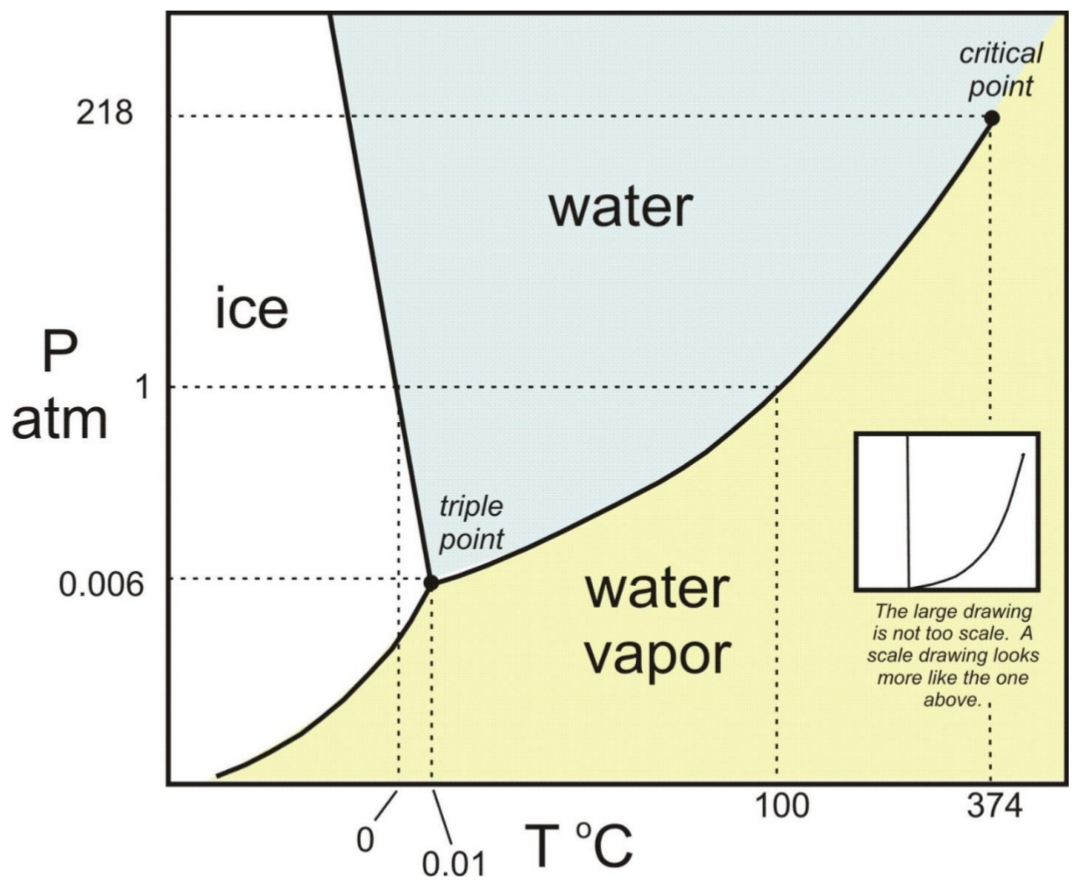
\includegraphics[width=0.7\linewidth]{img/wasser_aggregatszustaende}
	\caption{Aggregatzustände von Wasser}
	\label{fig:wasseraggregatszustaende}
\end{figure}


%-----------------------------------------------------------------------------
\section{TODO}
%-----------------------------------------------------------------------------


Druckabfall Rohrleitung: $\Delta p = \lambda(Re) \frac{\rho u^2}{2}\frac{l}{d}$

$Re = \frac{\rho u d}{\mu}$

$\mu$ = Viskosität

$\rho$ = Dichte

Zähigkeit = dynamische Viskosität


Laminare oder Turbulende ströhmung? 
Re < 2340 -> Laminar
	$\lambda(re) = 64/Re$
	
Re > 2340: Turbulent
	$\lambda(Re) = \frac{0.316}{Re^{1/4}}$

\subsubsection{Einheit Mol}

1 mol Wasser wiegt 18g.

\subsubsection{Allgemeine Gaskonstante}

\[
	N_A k_B = 8.314 \frac{J}{mol \cdot K}
\]

\subsubsection{Klassifizierung thermodynamische Systeme}

Was tauscht ''eine Box'' mit der Umgebung aus?


\begin{description}
	\item[Offen] Tauscht mit der Umgebung Energie und Masse aus
	\item[Geschlossen] Tauscht Energie mit Umgebung aus
	\item[Abgeschlossen] Kein Austausch mit UMgebung
	\item[Adiabatisch] Tauscht mechanische Arbeit mit der Umgebung aus (aber keine Wärme)
\end{description}

\subsubsection{Thermodynamische Begriffe}

\begin{description}
	\item[Thermodynamisches System] Abstraktion für ein reales System, welches Untersucht werden soll, Beispiele: Gastank, Ofen, die Erde
	\item[Thermodynamische Zustandsgrössen definieren das System] Druck, Stoffmenge (Anzahl Moleküle oder Anzahl Mol), Temperatur
	\item[Prozessgrössen beschreiben Prozesse] Wärme und Arbeit
	\item[Wärmelehre oder Thermodynamik] Alles was mit Wärme und Temperatur zu tun hat
	\item[Statistische Mechanik] Herleitung der Thermodynamik aus mikroskopischen Überlegungen, z.B. kinetische Gastheorie
\end{description}


\subsubsection{Zustandsgleichung: Druck, Temperatur, Volumen}


\[
	f(p, T, V) = 0
\]



\[
p V = N k_B T
\]


\begin{description}
	\item[$p$] Absolutdruck
	\item[$V$] Volumen	
	\item[$N$] Anzahl Molekühle
	\item[$T$] Temperatur in Kelvin
	\item[$k_B$] Wolfsmannkonstante
\end{description}

Zustandsgleichung: $\frac{pV}{T} = const.$

%TODO: Slide 5,6


$n$: Molzahl



%-------


\paragraph{Der erste Haptsatz der Thermodynamik:}

Energierhaltung $dU = \delta Q + \delta W$

\begin{description}
	\item[$U$] Innere Energie
	\item[$Q$] Wärme
	\item[$W$] Arbeit
\end{description}

\paragraph{Zweiter Haptsatz:}

Entropie kann nicht abnehmen.

\subsection{Wärmekapazität}

\[
	\delta Q \sim dT
\]

\subsubsection{Beispiel Wärmekapazität}

Wärmekapazität Wasser: $4.1868 kJ / kg K$

Wie viel Energie brauchen wir um 1g Wasser um $1^\circ$ C aufzuwärmen?
%TODO: Beispiel von Slide 19.
\[
SQ = 
\]





\subsubsection{Äquipartitionstheorem}

Wärmekapazität = 0.5 x Anzahl Freiheitsgrade x N x $k_B$

$C = \frac{f}{2}N k_B = \frac{f}{2} nR$

$C_m = \frac{f}{2} R$

$N$ Anzahl Atome


Körper mit gleicher Molzahl haben die gleiche Wärmekapazität


Bei kristalliner Festkörper:

Hohe Temperaturen: $C_{mv} = 3R$

Tiefe Temperaturen %TODO: Slide 24 Formel $C_{mv} = $

\paragraph{Gase}

Bei Gasen wird auch ein Teil der Aufwärm-Energie genutzt, um sich auszudehnen (falls möglich.)




\subsubsection{Phasenübergänge: Thermodynamische Phasen}

\begin{description}
	\item[Fest] Form und Volumen bestimmt
	\item[Flüssig] Bestimmtes Volumen
	\item[Gasförmig] Weder Form noch Volumen bestimmt.
	\item[(Plasma)] Ionisiertes Gas.
\end{description}

%TODO: Grafik seite 33

\subsubsection{Latente Wärme}


\[
Q_f = C_v \Delta T
\]


Bei einem Phasenübergang wird sehr viel Wärme aufgenommen oder abgegeben:

$ \frac{Q_s}{c_v}$

%todo: Tabelle Seite 39



\subsubsection{Dampfdruck}


Der Dampfdruck stellt sich ein, wenn Wasser und Luft im Gleichgewicht sind.

100\% Luftfeuchtigkeit bedeutet: $T = 20^\circ C \Rightarrow P_w = 23.4$ mbar Partialdruck


\subsubsection{Taupunkt}

Bei welcher Temperatur wäre die Luftfeuchtigkeit 100\%?


\subsubsection{Wärmeleitung}
Gesetz von Fourier: Nur Wärme, keine Masse

\paragraph{Wärmestromdichte} $j_Q = - \lambda \frac{dT}{dx}$


$[j_a] = \frac{W}{m^2}$


$[j] = \frac{W}{m^2}$

$[\lambda] = \frac{W}{m \cdot K}$

\paragraph{Wärmeleitungsgleichung} %TODO: Slide 4

\subsubsection{Wärmeübergang - Konvektion}
Wärme + Masse

Die Temperatur ändert sich sehr schnell in einer Grenzschicht. Dafür ist die Konvektion zuständig.

$j = \alpha (T_w - T)$

Wärmeübergangszahl $\alpha$

\paragraph{Beispiel: Wärmeleitung in einem elektronischen Bauteil}
%TODO: Slide 14




\subsubsection{Strahlung}
Stephan-Boltzmann


Jeder Körper > 0 K verliert Energie in Form von elektromagnetischer Strahlung

Die Strahlung ist proportional zu $T^4$ (Stefan-Boltzmann). Die Frequenzverteilung ist eine eindeutige Funktion der Temperatur (Planksches Strahlungsgesetz).

\paragraph{Strahlungsformel von Plank}

Planksche Konstante: $h = 6.626 \cdot 10^-43$

\[
	u(v,T)dv = \frac{hv}{e^{hv/k_BT} - 1} \frac{8\pi}{c^2} v^2 dv
\]

\begin{description}
	\item[$u$] Energiedichte in $\frac{J}{m^3}$
	\item[$v$] Frequenz
	\item[$T$] Temperatur
\end{description}

Atome können nur endliche Quentaen aufnehmen: $e_v = hv$


\paragraph{Elektromagnetische Strahlen}

Können alle perfekt mit der Maxwell-Gleichung beschrieben werden


Die Energie eines Photons: $E_{ph} = hv$. Bei Strahlung, welche Atome zerstören können, nennt man Ionisierende Strahlung.




\paragraph{Stefan-Boltzmann Gesetz}

Bei einer gewissen Temperatur, wie viel Energie geht mit der Fläche verloren.

$\sigma_{SB}$ ist die Stefan-Boltzmann Konstante: $=5.67 \cdot 10^-8 \frac{W}{m^2 K^4}$

Das totale Emissionsvermögen eines schwarzen Körpers ist:

\[
	K_s(T) = \sigma_{SB} T^4
\]

z.B: Wie warm wird eine Herdplatte: $P = \sigma_{SB} \cdot T^4 \cdot A$

 
\subsubsection{Entropie}

In einem geschlossenen System, bei dem das Volumen des Gases grösser wird, ändert sich der Druck. Die Temperatur ändert sich nicht.

$pV = nRT$ bei einem Idealen Gas

$U = \frac{3}{2} nRT$


\paragraph{Eigenschaften der Entropie}

Wärmezufuhr / Temperatur:
\[
	dS = \frac{dQ}{T}
\]

\subsubsection{Hauptsätze der Thermodynamik}

\begin{enumerate}
	\item Energierhaltung
	\item In einem geschlossenen System kann die Entropie nie abnehmen.
\end{enumerate}


\subsubsection{Wirkungsgrad}

Carnot-Wirkungsgrad:

\[
	\eta = 1 - \frac{T_L}{T_H}
\]



\end{document}